%%%%%%%%%%%%%%%%%%%%%%%%%%%%%%%%%%%%%%%%%%%%%%%%%%%%%%%%%%%%%%%%%%%%%%%%%%%%%%%

\chapter{PROPOSTA}

\textbf{[Que tal trocar isso para uma "definição do problema"?]}

\section{Dados}

A tabela \ref{table:bigdatasattypes} mostra os tipos de dados relevantes para a operação, a sua origem e o seu formato esperado, ignorando os dados provenientes da carga útil.

\begin{table}[!ht]
  \begin{center}
  \caption{Dados de Operação}
  \begin{tabular}{|c|C{5cm}|c|}
      \hline
      \bfseries Tipo de Dado &\bfseries Origem &\bfseries Formato \\
      \hline
      Sensores de bordo & Equipamentos no satélite & Tabelas, CSV \\
      \hline
	  Registros do Computador & Computador de Bordo & Texto (\textit{Logs}) \\
      \hline
	  Multimídia & Câmeras & MP4, JPG, RAW \\
      \hline
	  Parâmetros orbitais & Operação, Rastreio & TLE, texto, tabelas \\
      \hline
	  Documentação associada & Operadores, engenharia & Texto (Word, Excel) \\
      \hline
	  Clima Espacial & Sensores no solo ou espaço & Texto, tabelas, avisos \\
      \hline
	  \textit{Situational Awareness} & Radares, US-STRACOM, etc & Texto, tabelas, avisos \\
      \hline
  \end{tabular}
  \end{center}
  \FONTE{Adaptado de~\cite{zhangBigDataFramework2017}}
  \label{table:bigdatasattypes}
\end{table}

Para este trabalho, apenas os dados vindos de sensores de bordo serão considerados. Os outros dados nesta tabela poderiam ser considerados para uma \textit{Data Warehouse} mais completa, pois um cubo de dados pode ser formado sobre quaisquer um desses dados.

Por exemplo, um cubo de dados textual poderia ser feito sobre os documentos associados a operação, como o CONOPS, tabelas de telecomandos e documentação de engenharia de sistemas para facilitar a análise da documentação sendo gerada pelo satélite. Um cubo multimídia poderia ser gerado sobre os dados multimídia tirados pelas câmeras do satélite para correlacionar com os dados gerados pelos sensores, e assim em diante. Alguns exemplos de cubos possíveis de serem feitos estão em~\cite{silva:2015:abordagensParaCubo}.

Esta lista não é exaustiva, e pode incluir dados da carga útil caso sejam relevantes para a análise em questão, como ajudar na georeferênciação de imagens tiradas pelo satélite.

\section{Fluxo dos Dados de Operação}

A figura~\ref{fig:bigdataflow} demonstra o fluxo de dados esperado de uma arquitetura de \textit{Big Data}.

\begin{figure}[ht]
	\caption{Fluxo de dados em uma arquitetura de Big Data}
	\vspace{6mm}
	\begin{center}
		\resizebox{15cm}{!}{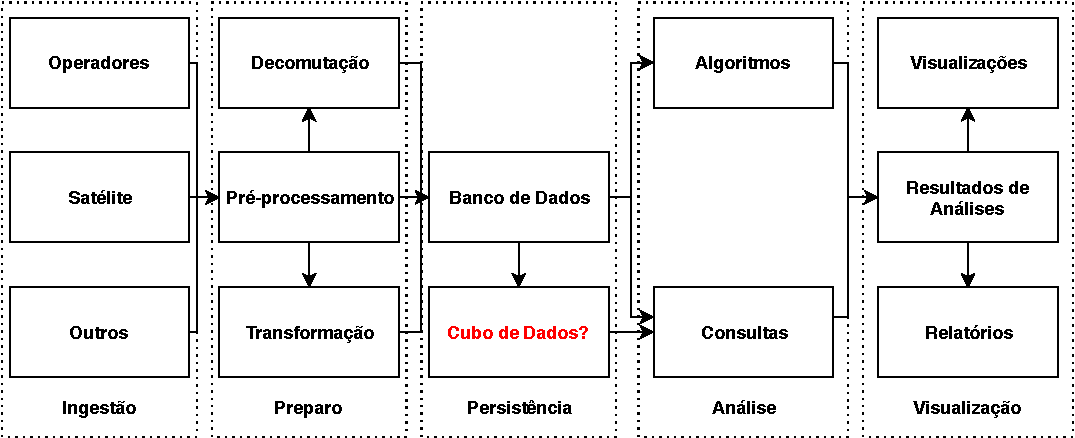
\includegraphics{Figuras/BigDataFlow.pdf}}
	\end{center}
	\vspace{2mm}
	\legenda{}
	\FONTE{Adaptado de~\cite{zhangBigDataFramework2017}}.
	\label{fig:bigdataflow}
\end{figure}

\section{Arquitetura de um Cubo de Dados}

A figura~\ref{fig:cubearch} demonstra a divisão em 4 partes de uma estrutura de Cubo de Dados.

\begin{figure}[ht]
	\caption{Arquitetura de um cubo de dados}
	\vspace{6mm}
	\begin{center}
		\resizebox{10cm}{!}{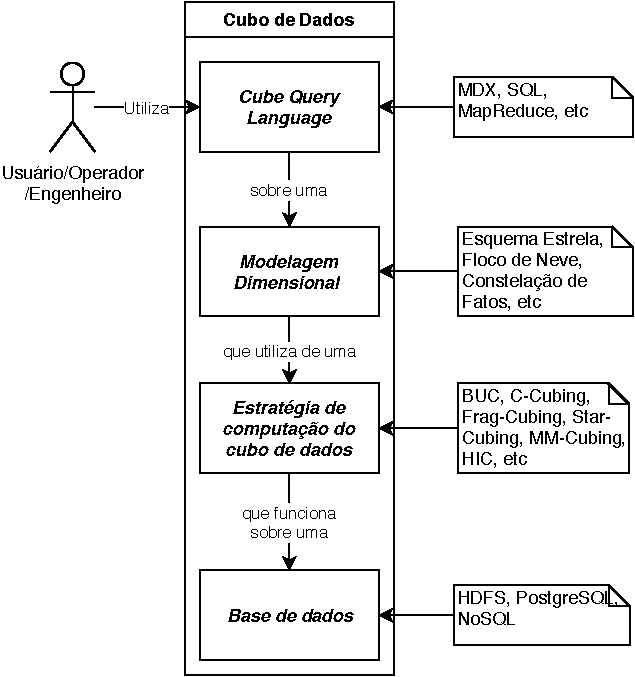
\includegraphics{Figuras/DataCubeArchitecture.pdf}}
	\end{center}
	\vspace{2mm}
	\legenda{}
	\FONTE{Autor (2019)}.
	\label{fig:cubearch}
\end{figure}

Esta proposta foca apenas na proposição de um algoritmo de computação do cubo de dados mais apropriado, utilizando das outras seções quando elas vão se tornando necessárias.

